\documentclass[11pt,letterpaper]{article}

\usepackage{graphicx}
\graphicspath{{./figures/}}

\usepackage[margin=1in,paperheight=11in,paperwidth=8.5in]{geometry}
\usepackage{fancyhdr}
\usepackage{subcaption}
\pagestyle{fancy}
\lhead{DRAFT}

\usepackage{lscape}

\usepackage{algorithm}
\usepackage{algpseudocode}   %[noend]
\usepackage{array}
\usepackage{xcolor,colortbl}
\usepackage{textcomp}

\newcolumntype{L}[1]{>{\raggedright\let\newline\\\arraybackslash\hspace{0pt}}m{#1}}
\newcolumntype{C}[1]{>{\centering\let\newline\\\arraybackslash\hspace{0pt}}m{#1}}
\newcolumntype{R}[1]{>{\raggedleft\let\newline\\\arraybackslash\hspace{0pt}}m{#1}}


%-------------------------------------
\newcommand{\figref}[1]{Figure~\ref{#1}}
\newcommand{\eqref}[1]{Eq.~(\ref{#1})}
\newcommand{\ttt}{\texttt}
\newcommand{\reg}{\textsuperscript{\textregistered}}
%-------------------------------------
\title{Formulation and Modifications for SolTrace Speed Improvement}
\author{Mike Wagner \\ Tim Wendelin }
\date{\today}

\setlength{\parskip}{1ex}

\begin{document}

\maketitle

\vspace{0.5\textheight}

\centering

\includegraphics[width=0.5\linewidth]{nrel-logo}

\raggedright

\clearpage

%\section{Background}

\section{SolTrace Hierarchy}

SolTrace consists of a user interface (UI) and an underlying computation core, called ``coretrace''. 
The UI provides input forms where the user can set simulation parameters, construct geometries, and configure optical and surface characteristics. 
Several data structures are instantiated and maintained by the interface, and these structures are used to construct the data structures that are required by coretrace to run a simulation. 
Because coretrace can be called independently from the UI via the application programming interface (API), or it can be called in a multi-threading environment, the structures used by the interface must be separate from those used by coretrace. 
Consequently, the UI data structures duplicate much of the coretrace structure. 

When coretrace is invoked, the UI maps user input to the coretrace structure via the coretrace API. The general layout of the interface with respect to its data structures and coretrace is shown in \figref{fig:app-layout}. 

\begin{figure}[tbp]
\centering
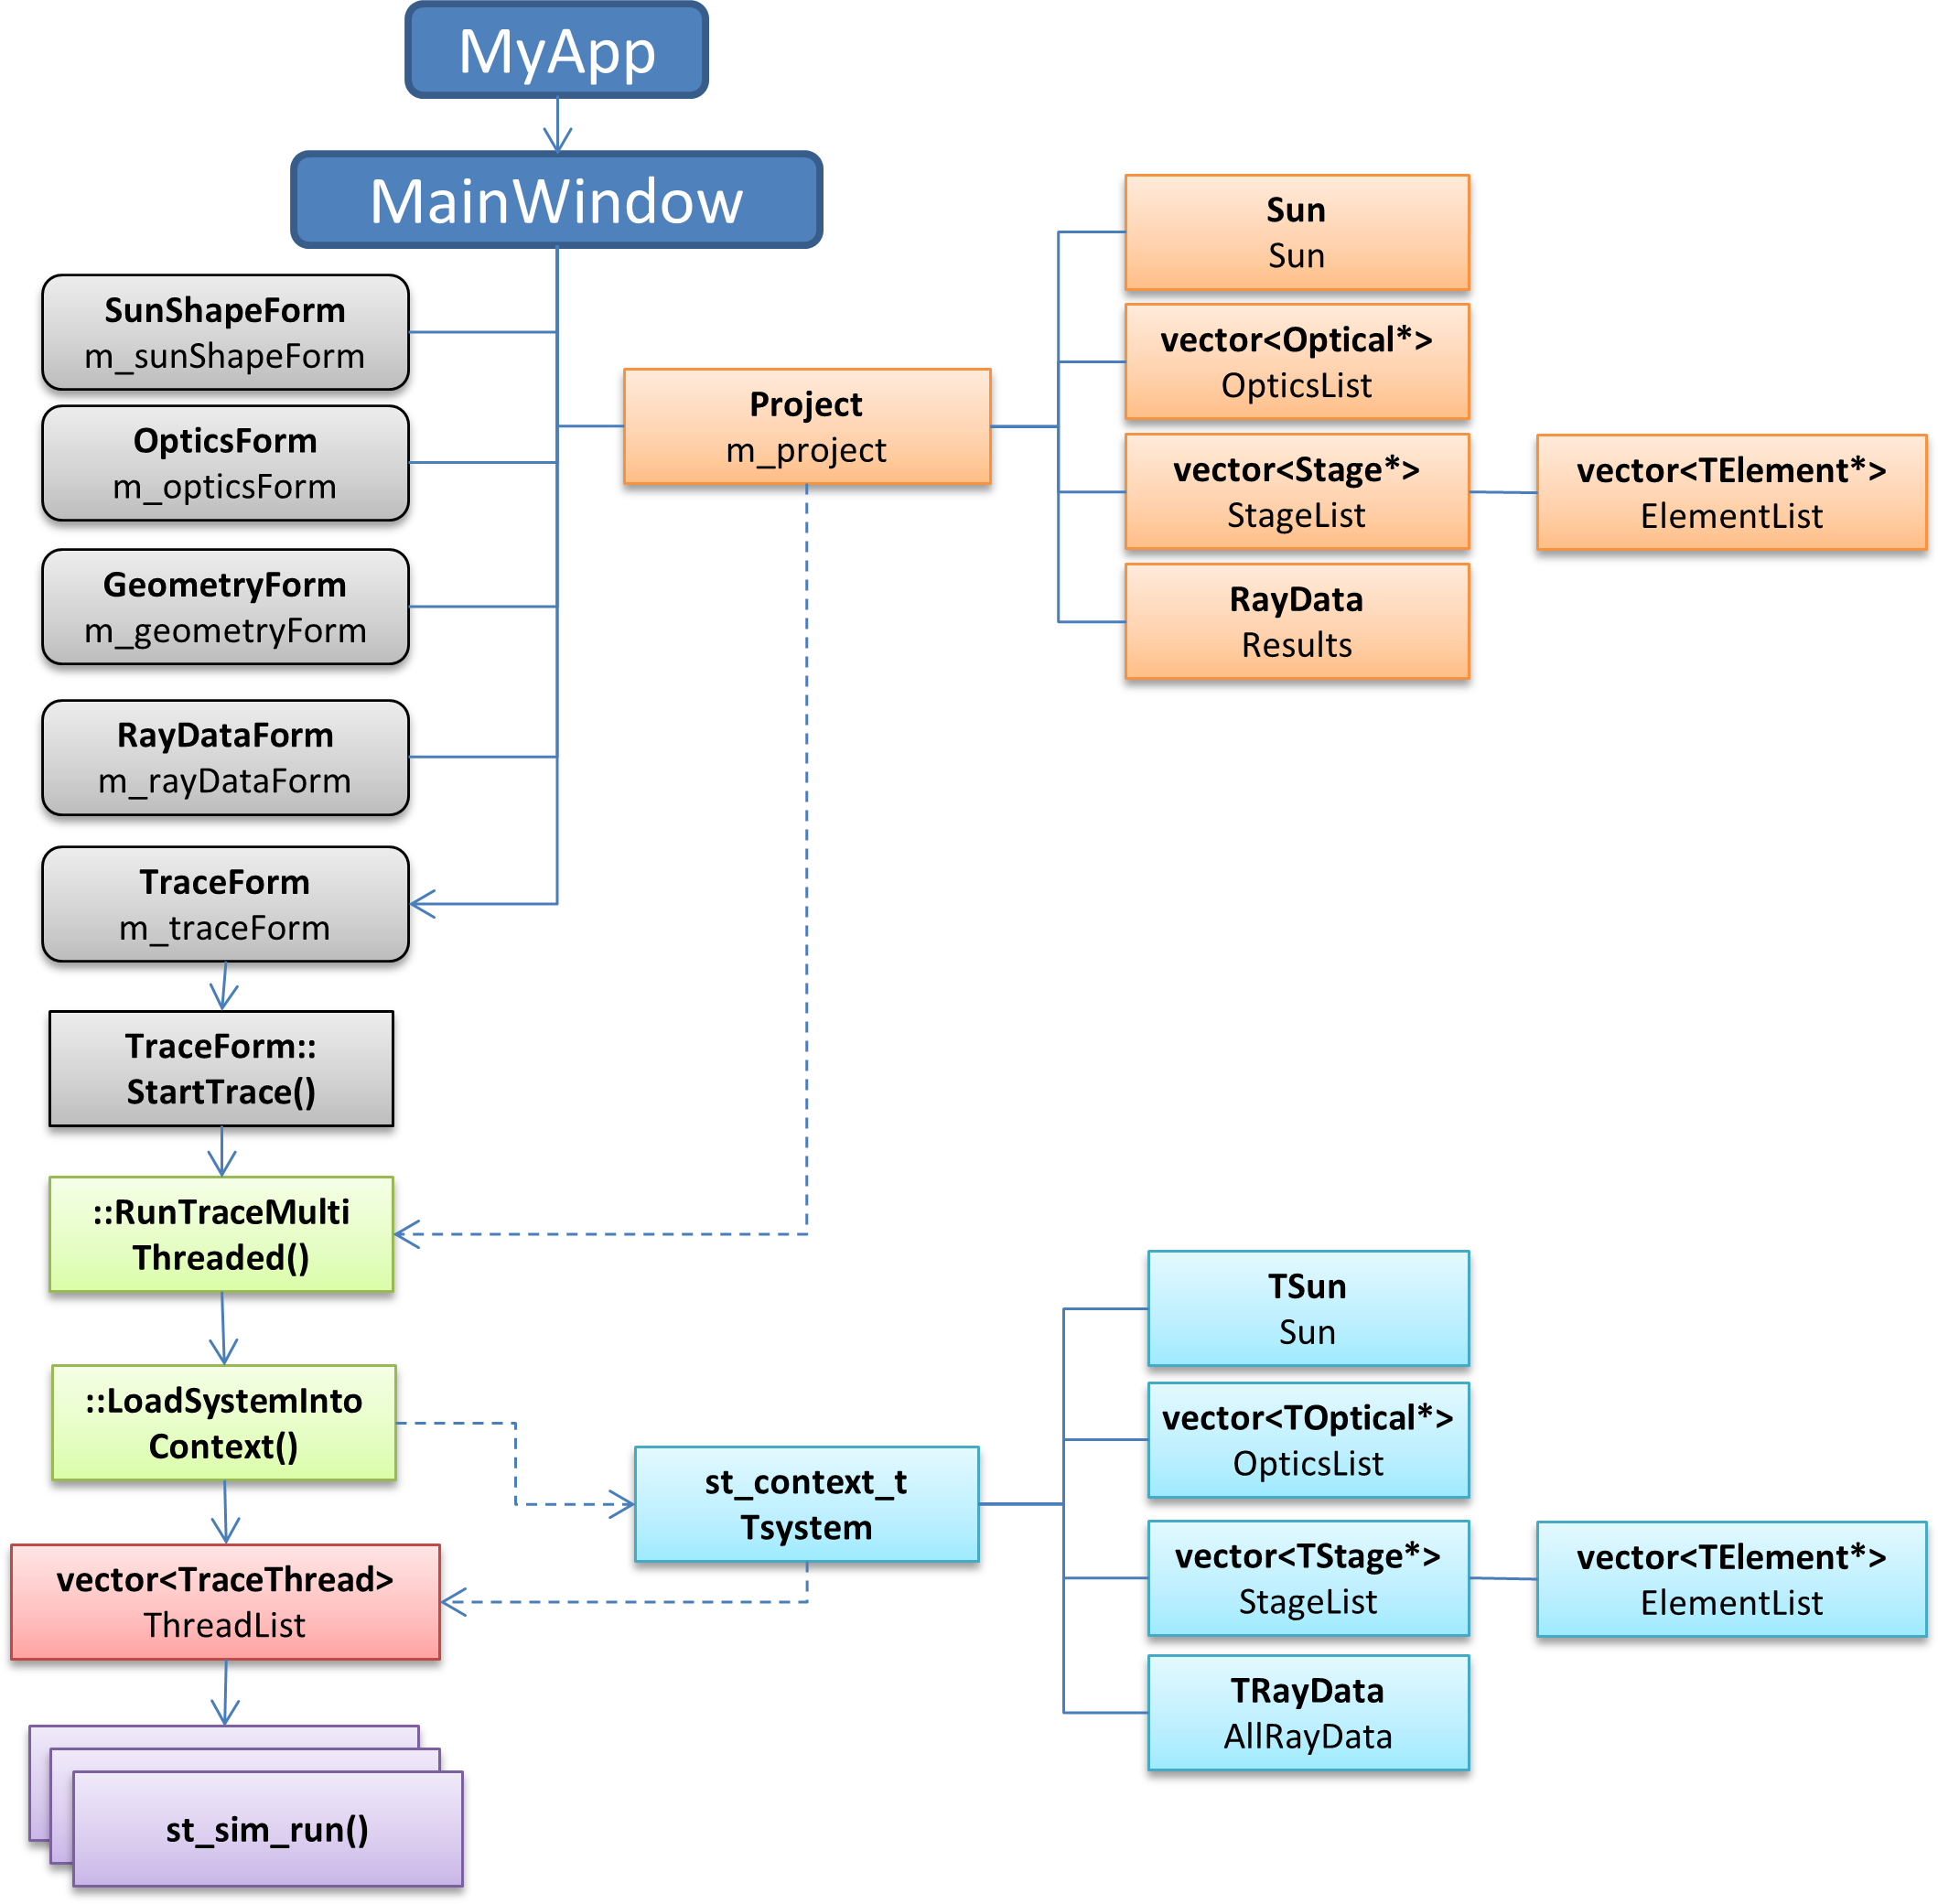
\includegraphics[width=\textwidth]{app-layout}
\caption{UI layout, data structures, and relationship to coretrace.}
\label{fig:app-layout}
\end{figure}

The SolTrace data flow process begins with initialization of the main program and interface window (MyApp and MainWindow). 
The MainWindow instance creates instances of each interface page that become members of the MainWindow object. 
In \figref{fig:app-layout}, class names are indicated in boldface at the top of each box while the member name given to an instance of the class is given in plain font at the bottom of each box. 
Shown in gray are UI form objects that provide interfacing functionality. 
Shown in orange are the data structures that are constructed from the input that the user provides. 
The primary data structure is of type {\bf Project} and has members {\bf SunC}, {\bf Optical}, {\bf Stage}, and {\bf RayData}. 
Structures that have multiple potential instances are collected in a C++ ``vector'' and are instantiated dynamically. 
The {\bf Stage} data structure also has a member structure of individual optical elements of type {\bf TElement}. 

When a simulation is executed, the {\bf Project} data structure is passed to the \texttt{RunTraceMultiThreaded()} function that prepares the simulation. 
Next, the data structure is mapped onto the analogous coretrace data structure shown in blue. 
If multiple threads are required, the {\bf st\_context\_t} structure is multiply instantiated.  
The resulting ThreadList objects each call their respective {\bf st\_sim\_run()} functions where the {\bf Trace()} algorithm is subsequently executed. 

%\section{Trace() Algorithm Layout}




\begin{landscape}
\begin{figure}[p]
\centering
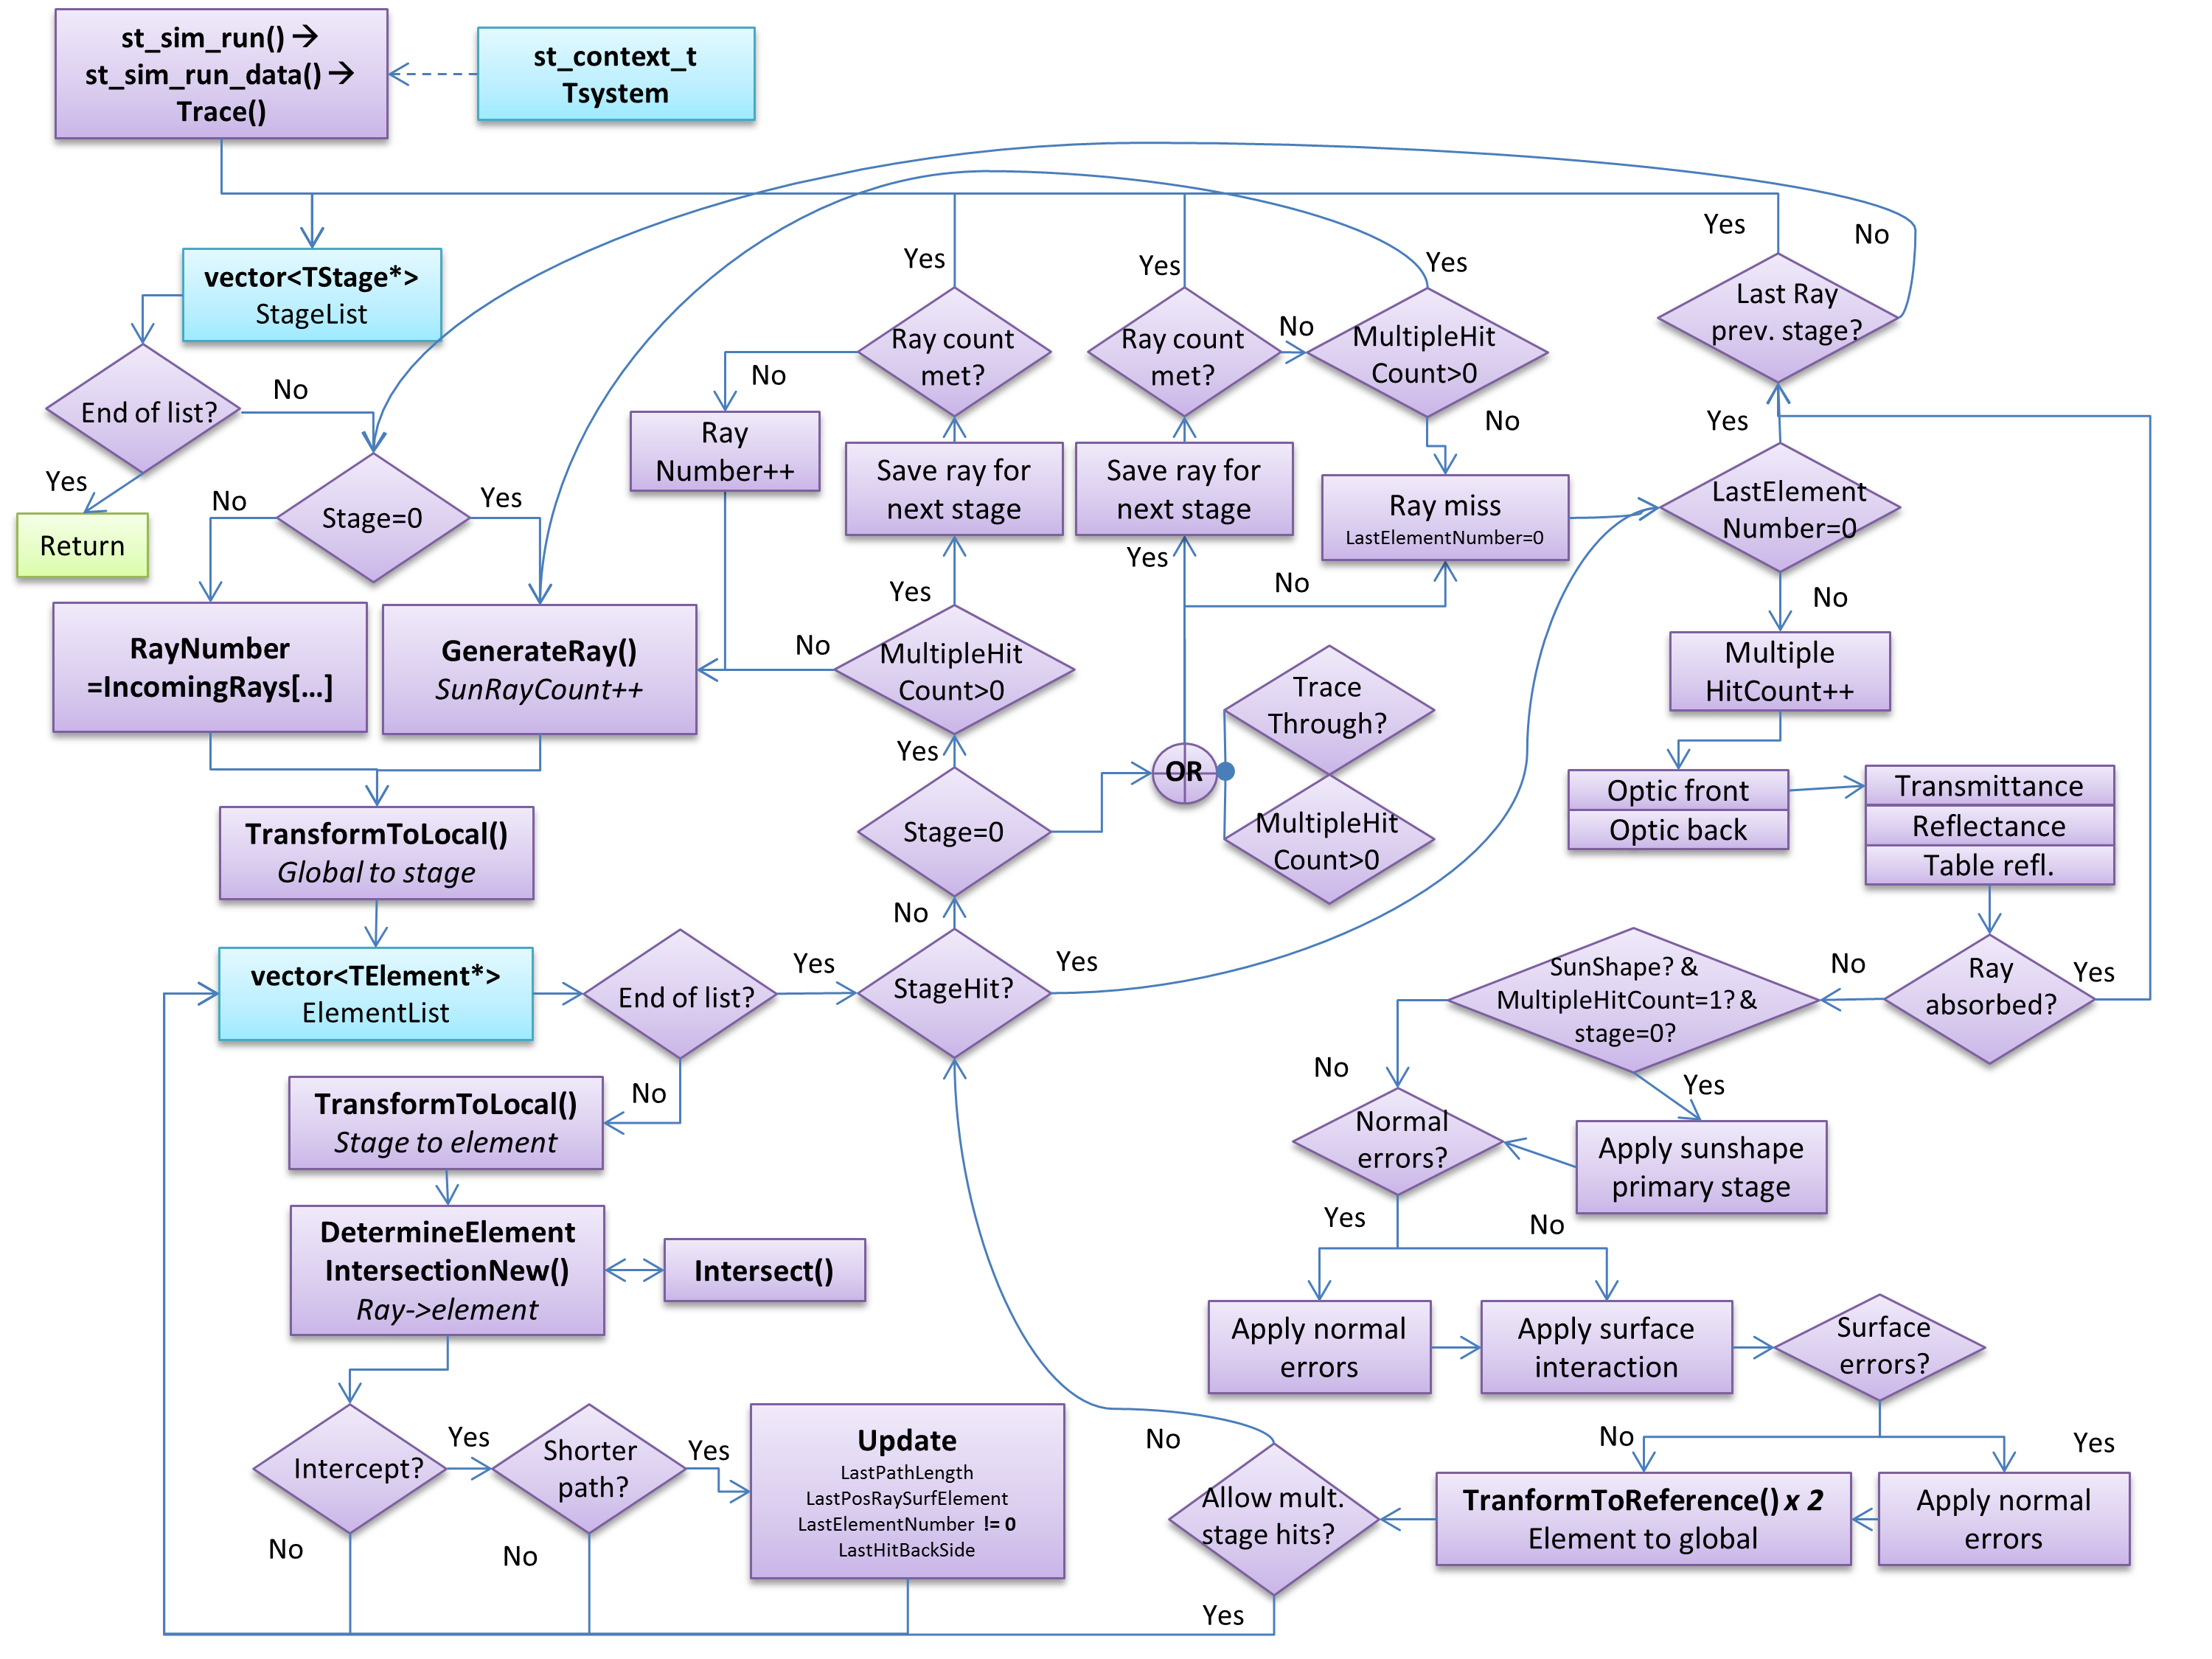
\includegraphics[height=0.92\textwidth]{coretrace-layout}	%,angle=90
\caption{}
\label{fig:coretrace-layout}
\end{figure}
\end{landscape}

%\section{Reverse Tracing and Emitting Surfaces}






\section{Dynamic Grouping Methodology and Formulation}

\subsection{Background}
As outlined in Figure~\ref{fig:coretrace-layout}, SolTrace generates solar rays with a vector defined by the position of the sun-shape profile and at random positions within a rectangular box surrounding all elements within the first stage. 
This procedure mimics the physical behavior of photons striking a region of interest, where each ray has a unit vector whose components depend on the position of the sun and a probability density function describing the apparent shape of the sun. 
SolTrace identifies the intersection between a given ray and an element by testing whether a randomly generated ray collides with any element in the first stage. 
Because SolTrace is a generalized ray-tracing tool, it is possible that a ray's projected path may either intersect multiple elements, a single element, or no elements at all. 
Consequently, each generated ray must be tested against each element in the stage to ensure that an intersection is not in fact preempted by another intersection with an element that shadows the first positive test. 

Power tower systems are relatively sparse in terms of land occupancy fraction -- that is, the ratio of mirror surface area to total land area inside the SolTrace bounding box is relatively small. 
A randomly generated ray is therefore not likely to strike any element in the stage, but this fact can only be determined after testing each element in the stage for intersection. 

Once a valid ray-element intersection has been detected, the reflected ray may potentially strike another element within the first stage, so a second exhaustive series of intersection tests must be executed. 
Any number of first-stage ray intersections is possible for a generalized geometry, but for power tower systems, multiple first-stage intersections is most likely due to inter-heliostat blocking (i.e., a ray reflects off a first heliostat and then strikes the back of an adjacent heliostat). 
%Each ray reflection in the first stage results in a subsequent requirement to test all elements in the stage for another intersection. 

Power tower systems with tens or hundreds of thousands of geometrical elements in the first stage therefore incur a tremendous computational expense to identify sun rays that will ultimately be reflected out of the stage toward the receiver. 
For a typical heliostat field with 100,000 first-stage elements, only 1 in 4-5 rays strikes an element, and each successful ray requires no less than two full passes through the list of elements for intersection testing. 
In total, each ray that reaches the receiver for the typical case requires somewhere between 200,000 - 600,000 intersection tests. 
As a result, a corresponding ray-trace simulation running 1M rays (receiver hits) on a dual-core (4 thread) laptop with Intel i7 2.6 GHz processors can require 4 hours or more to complete. 

In this paper, we develop a methodology to significantly reduce computation time while preserving the fidelity and robustness of the ray-tracing approach in SolTrace. 
The premise underlying the speed improvement is that the primary computational expense lies in testing each stage element for intersection when in fact only certain elements that are near the position of the randomly generated solar ray need to be tested for intersection. 
By substantially reducing the number of elements that are in the hit-test loop, reflected rays can very quickly be identified. 
However, a method must first be developed for quickly identifying heliostats that may potentially interact with a ray or the computational expense will simply shift from intersection testing to proximity testing and sorting. 

\subsection{Model premise and conceptual description}
While SolTrace provides general ray-tracing functionality, several problem features provide an opportunity for speed enhancement. 
Firstly, the elements within a particular geometry are fixed in place throughout the simulation. 
Secondly, rays originate from a relatively narrow angular window such that incoming rays are virtually collimated. 
Lastly, (for point focus systems such as power towers) light is reflected toward a narrow spatial region, and light that is not reflected toward this region is not of particular interest because it has been ``lost'' from the system. 

The speed improvement technique works by creating localized groups of elements, a small subset of which are retrieved for intersection testing based on the position of the random sun ray.  
Groups are generated before the ray-trace simulation begins, and the groups must be developed such that an incoming ray could plausibly (i.e., without knowing the exact position of the ray) strike any element in the group. 
The difficulty in developing meaningful groups lies in the fact that geometrical elements exist in three dimensional space, as shown for a randomly generated element field in Figure~\ref{fig:proj} (left). 
Here, assume that sun rays originate from a narrow window around the ``camera position'' of the Figure~\ref{fig:proj} plot. 
It is apparent that an element may interdict a sun ray from striking another element that is not close in proximity in $x,y,z$ space. 
Therefore, grouping of elements based on $x,y,z$ proximity is not generally meaningful. 

Instead, elements are grouped by their projection onto the plane normal to the sun vector, as illustrated in Figure~\ref{fig:proj}~(right). 
In this view, the coordinates of each element are expressed in two dimensions, and proximity in the transform space is meaningful in anticipating element-to-element interactions. 

\begin{figure}[htb]
\centering
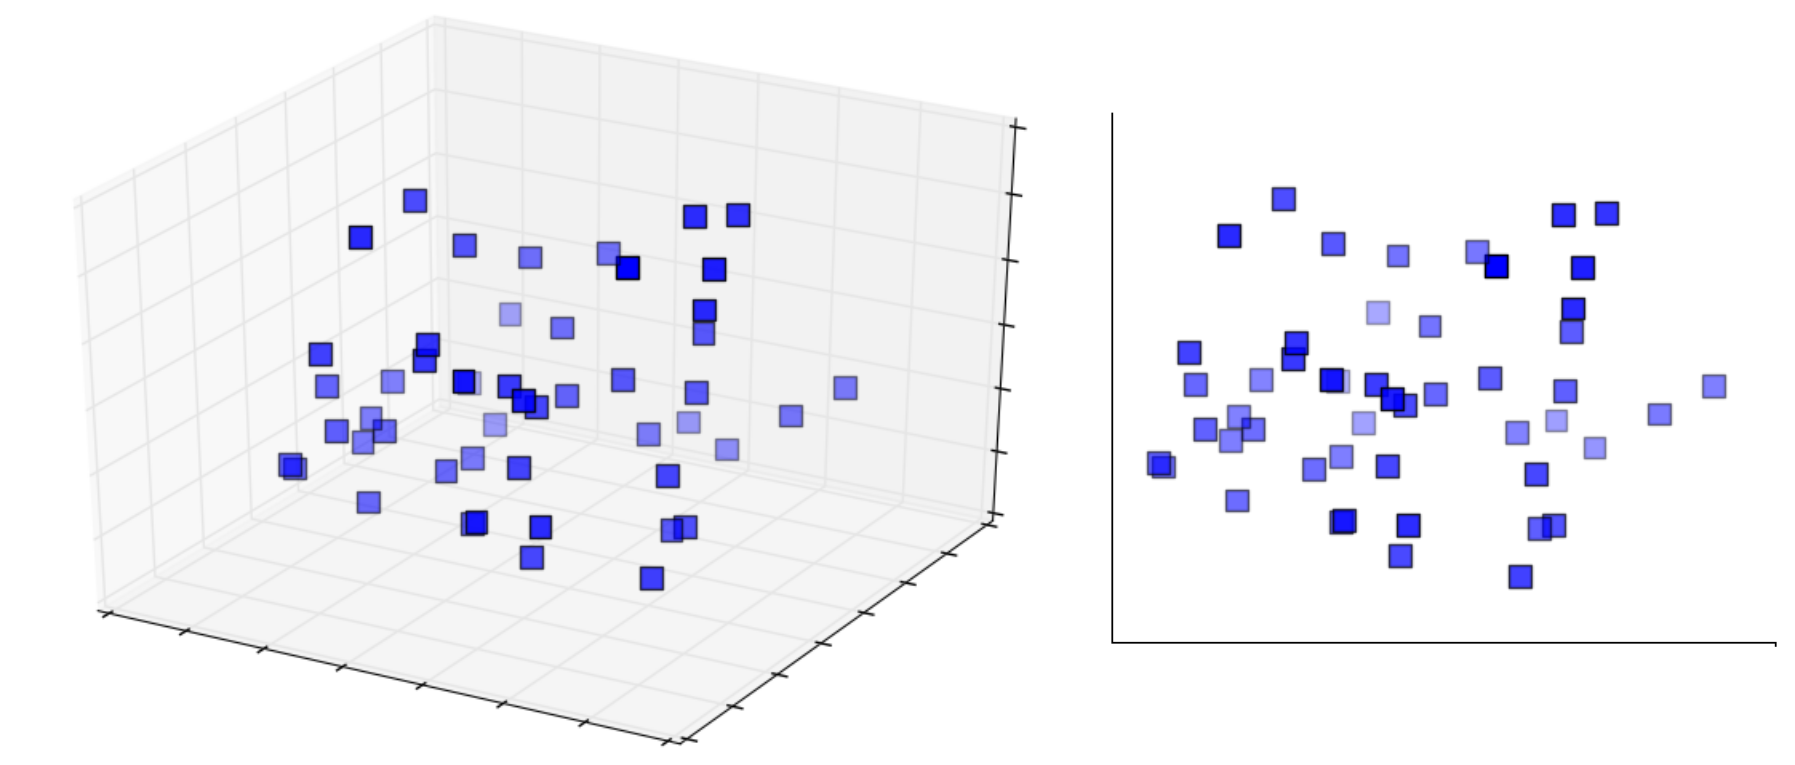
\includegraphics[width=\linewidth]{projection-h3}
\caption{A random set of elements shown in 3D space (left) and projected onto a 2D plane whose normal vector is the sun vector (right).}
\label{fig:proj}
\end{figure}

Elements are grouped into small zones that are sufficiently large to contain the largest local element, but small enough that the number of elements in each group is minimized. 
Zones are not necessarily uniform in size, but are constructed based on the position and size of the local elements. 
The location of each zone is specified using a binary address that corresponds to halving subdivisions in each coordinate dimension. 
The location code specifies whether the position in question is on the positive side (1) or negative side (0) of the subdividing line, and alternating characters in the code correspond to alternating coordinate system dimensions. 
For example, a zone location code of ``1101'' indicates a zone (in cartesian coordinates) that is on the positive side of an x-axis subdivision, then positive of a y-axis subdivision, then negative of x-axis, then positive of y-axis, as shown in Figure~\ref{fig:cart-map}. 
Note that as the length of the code increases, the precision of the specified zone increases. 

\begin{figure}
[htb]
\centering

\includegraphics[width=0.35\linewidth]{cart-map}
\caption{Zone position corresponding to code ``1101'' in a cartesian mesh.}
\label{fig:cart-map}
\end{figure}

The discussion to this point has presented the motivation and background for sorting elements based on their projection onto the sun normal vector plane. 
This projection is beneficial in quickly identifying local groups for potential intersection with a sun ray, but once the element is reflected, the initial grouping is no longer relevant. 
However, point focus systems concentrate light toward a small region, and a similar projection can be made in polar coordinates to identify elements that might potentially block reflected light. 
The polar projection places the ``camera view'' at the receiver position, and groups heliostats based on proximity from this perspective. 
Figure~\ref{fig:meshes} shows an example of the sun projection mesh (Fig.~\ref{fig:full-mesh}) and of the receiver projection mesh (Fig.~\ref{fig:polar-mesh}). 

\begin{figure}[htb]
\begin{subfigure}{0.48\linewidth}
	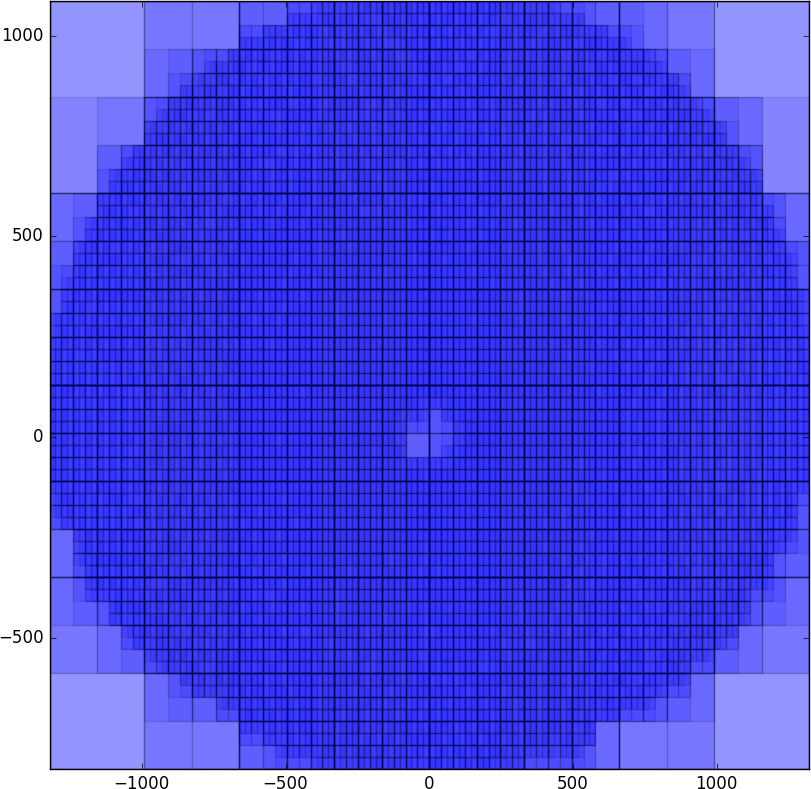
\includegraphics[width=\linewidth]{full-mesh}
	\caption{Sun-projection mesh in cartesian coordinates.}
	\label{fig:full-mesh}
\end{subfigure}
~
\begin{subfigure}{0.48\linewidth}
	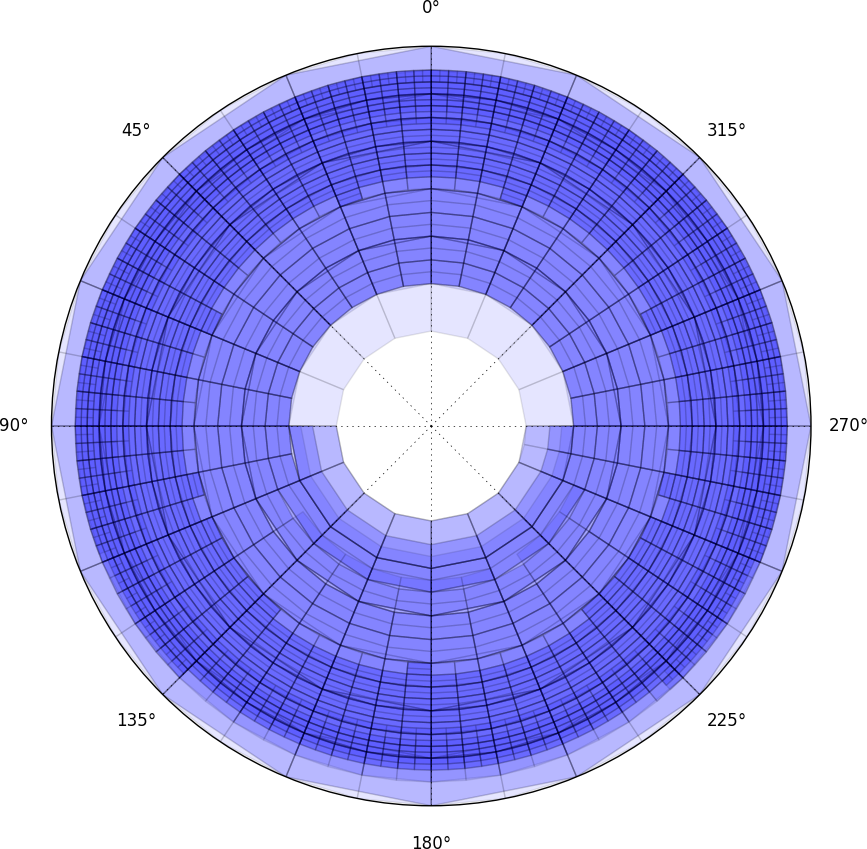
\includegraphics[width=\linewidth]{polar-mesh}
	\caption{Receiver-projection mesh in polar coordinates.}
	\label{fig:polar-mesh}
\end{subfigure}
\caption{}
\label{fig:meshes}
\end{figure}

Figure~\ref{fig:polar-mesh} plots the mesh from the view of the receiver, where a view downward corresponds to the center region of the plot, and a view toward the horizon corresponds to the outer radial positions on the plot. 
The finer meshing near the perimeter of the plot captures the effect of the smaller apparent size of the heliostats near the horizon (that are farther away in the field), and the smaller azimuthal angular span occupied by elements near the equatorial latitudes of a polar coordinate system. The outer radius of the plot is the horizon. 
%
Note that mesh elements are variable in size, and the mesh is densest in regions where heliostat elements are present.

\subsubsection{Zone attributes}
Each zone is defined by a unique binary code, and the zones are constructed recursively (i.e., the function that subdivides a zone calls itself until the subdivision requirements have been met), and any particular zone may have up to two child zones. 
A zone may alternatively have no child zones but instead contain a list of elements that lie within it.
To understand this structure, reconsider the example mesh in Figure~\ref{fig:cart-map} above. 
Here, there are five zone instances: 
\begin{enumerate} 
	\item the full bounding box, 
	\item the positive-x half of (1), 
	\item the positive-y half of (2), which is the upper-right quarter of (1),
	\item the negative-x half of (3),
	\item the positive-y half of (4).
\end{enumerate}

By convention, only terminal nodes (node \#5 in this example) can contain elements, whereas intermediate nodes contain children nodes. 
Terminal nodes may be empty if a region does not contain elements. 


\subsubsection{Parsing the zonal mesh}
%The following section provides 
When a random sun ray is generated, the position of the ray in the cartesian projection is translated into a binary code according to the method previously discussed. 
The algorithm parses the zonal mesh, following the map of subdivisions in accordance with the sun ray positional code. 
When an address leads to a terminal zone, any elements contained are subsequently tested for intersection with the ray. 
Elements that are positioned within a particular zone may extend into a neighboring zone, so all adjacent zones are also identified and their elements tested for intersection. 


\subsection{Formulation}

The element grouping method provides two main algorithms -- one for initial mesh development and another for retrieval of elements based on a ray location. 
Note that the methods are not dependent on the coordinate system used. 

\subsubsection{Mesh definition}

The mesh is developed {\sl ad hoc} by subdividing the field as elements are added with the following procedure. 
First, the mesh starts as a single node encompassing the entire bounding area under consideration. 
The elements are sorted according to their apparent size in the coordinate system. For cartesian coordinates, the apparent size is equal to the physical element size (maximum diameter). 
Each element is added to the mesh in sequence, and the mesh subdivides until the resulting zone size would be smaller after subdivision than the element that is being added. 
At this point, the node is flagged as a terminal node, and the element is added to the list of local elements. 

For subsequent element additions, a terminal node cannot be subdivided, so an element that is smaller than one that has already been added to a terminal node will not cause additional subdivision. 
This process creates a ``tree'' structure, where branches from a given node correspond to smaller subdivided nodes within the ``parent'' node. 
When a subdivision takes place, only the half of the subdivision containing the new element will have a new node created. 
This maintains a minimally sparse tree. 
%
After a number of elements have been added, further additions traverse the existing tree, only creating new nodes as needed where none have previously been defined.

The final step in defining the mesh is to post-process each element to add neighboring elements to the list of those checked when a ray strikes a zone. 
This is done by testing for the existence of neighbor zones that are offset by $\pm 1$ in each coordinate direction in the binary code.
Algorithm~\ref{alg:mesh} shows pseudo-code for generation of the mesh. 

\begin{algorithm}
\small
\caption{~~Mesh construction}
\label{alg:mesh}
\begin{algorithmic}[1]
\State \Call{AddElement}{$\ttt{head node}, \ttt{element location code}, \ttt{0}, \ttt{element}$} 
%
\Procedure{AddElement}{$\ttt{node}, \ttt{code}, \ttt{index}, \ttt{element}$}
\State $x_0$ is lower $x$-direction zone limit
\State $x_1$ is upper $x$-direction zone limit
\State $x_c = \frac{x_0 + x_1}{2}$ 
\State $y_0$ is lower $y$-direction zone limit
\State $y_1$ is upper $y$-direction zone limit
\State $y_c = \frac{y_0 + y_1}{2}$ 
\State $D_{el}$ is element's apparent diameter
%\State $\ttt{SplitUpper}$ is {\sl true} if $\ttt{code}[\ttt{index}] == 1$
%
\If{ $\ttt{node}$ is terminal {\bf or} $\ttt{index}$ is past the end of $\ttt{code}$ }
	\State Add $\ttt{element}$ to node's element list; Flag zone as terminal
	\State \Return
\EndIf
%
\If{ Current dimension is $x$ }
	\State $W_{zone,x} = \frac{x_1 - x_0}{2}$ 
	\State $W_{zone,y} = \frac{y_1 - y_0}{2}$
	%
	\If{ $D_{el} > W_{zone,x}$ }
		\If{ A child node does \textbf{not} exist in the proposed split direction}
			\State Create a new node $\ttt{node}^\prime$
			%
			\If{$\ttt{code}[\ttt{index}] == 1$}  \Comment{Splitting in the positive direction}
				\State New node range is $x_0 = c_x$, $x_1 = x_1$, $y_0 = y_0$, $y_1 = y_1$
				\State \Call{AddElement}{$\ttt{node}^\prime, \ttt{code}, \ttt{index}+1, \ttt{element}$}
				\State \Return
			\Else
				\State New node range is $x_0 = x_0$, $x_1 = x_c$, $y_0 = y_0$, $y_1 = y_1$
				\State \Call{AddElement}{$\ttt{node}^\prime, \ttt{code}, \ttt{index}+1, \ttt{element}$}
				\State \Return
			\EndIf
		\Else
			\State \Call{AddElement}{$\ttt{Existing node}, \ttt{code}, \ttt{index}+1, \ttt{element}$}
			\State \Return
		\EndIf
	\Else
		\State A split is not allowed in the $x$ direction, but check for allowed splits in the $y$ direction
		\If{ $D_{el} > W_{zone,y}$ }
			\If{ A child node does \textbf{not} exist }
				\State Create a new node $\ttt{node}^\prime$
				\State New node range is $x_0 = x_0$, $x_1 = x_1$, $y_0 = y_0$, $y_1 = y_1$
				\State \Call{AddElement}{$\ttt{node}^\prime, \ttt{code}, \ttt{index}+1, \ttt{element}$}
				\State \Return
			\Else
				\State \Call{AddElement}{$\ttt{Existing node}, \ttt{code}, \ttt{index}+1, \ttt{element}$}
				\State \Return
			\EndIf
		\Else
			\State Add $\ttt{element}$ to node's element list; Flag zone as terminal
			\State \Return
		\EndIf	
	\EndIf
	%
\Else
	\State ... Replicate algorithm for $x$ dimension, swapping $x$ and $y$ terms
\EndIf
\EndProcedure
\end{algorithmic}
\end{algorithm}




\subsubsection{Zone retrieval}

Given a particular ray location, retrieving the corresponding zone is fairly straightforward using a recursive algorithm. 
The ray position is first expressed as a binary code, and this code implicitly provides instructions on how to traverse the tree mesh developed in the previous subsection.
The code characters are defined according to Table~\ref{tab:code}. 
\begin{table}[htb]
\centering
\small
\caption{Characters contained in a location code}
\label{tab:code}
\begin{tabular}{c|L{0.6\linewidth}}
{\bf Character} & {\bf Description} \\
\hline
1	& Traverse along the positive direction	subdivision \\
0	& Traverse along the negative direction subdivision	\\
x	& The current node does not subdivide in the specified dimension, continue to the next dimension	\\
t	& The current node is terminal and can contain data	\\
\end{tabular}
\end{table}

To retrieve an element, a code is passed to the processing algorithm. 
The algorithm inspects the code at the first character. 
If the character equals $1$, the algorithm calls itself with reference to the positive direction child node, and if $0$, with reference to the negative direction child node. 
This recursive call increments through the code, calling the appropriate child along the way. 
If the character is $x$, only one child is available and it is called recursively. 
If the character is $t$, or if the requested child ($1$, $0$, or $x$ is not defined, the algorithm finally returns all the way back up through the recursive call tree with a reference to the terminal node (or a null reference if no node exists). 
This algorithm is computationally efficient and covers the various cases introduced by nonuniform zone size, sparse meshing, variable quantities of elements in each zone, and independence from the coordinate system that is used. 
The algorithm is summarized in pseudo-code in Algorithm \ref{alg:fcpsuedo}.


\begin{algorithm}
\small
\caption{~~Zone retrieval}
\label{alg:fcpsuedo}
\begin{algorithmic}[1]
\Procedure{Process}{$\ttt{node}, \ttt{code}, \ttt{index}$}
\State $c = code[index]$ \Comment{the current character equals the code string at the index}
\If{$c == 1$}
	\State \Return \Call{Process}{$\ttt{child node 1}, \ttt{code}, \ttt{index+1}$}
\ElsIf{$c == 0$}
	\State \Return \Call{Process}{$\ttt{child node 0}, \ttt{code}, \ttt{index+1}$}
\ElsIf{$c == x$}
	\State \Return \Call{Process}{$\ttt{child node}, \ttt{code}, \ttt{index+1}$}
\Else \Comment{~ ($c == t$, terminal node)}
	\State \Return {\sl Address of this node}
\EndIf
\EndProcedure
\end{algorithmic}
\end{algorithm}





\subsection{Results}

The speed improvement algorithm was tested for a variety of power tower systems to demonstrate the flexibility of the methodology. 
The cases that were investigated are summarized in Table~\ref{tab:cases}. 


%1e5 rays
Each simulation was executed with 100,000 receiver ray intersections using 4 threads on an Intel\reg Xeon\reg 2.4 GHz processors running Windows Server 2012\reg (x64 architecture). 
Although the machine on which the simulations were executed is capable of up to 22 parallel threads, we limited the simulation to 4 threads to emulate the performance of a typical laptop computer, which at the time of writing contains a dual-core processor with up to 4 threads. 
The values reported are from a single simulation, although in reality there is a distribution of run times with some negligibly small standard deviation. 
Field layouts for cases 1, 4, 5, and 6 are shown in Figure~\ref{fig:cases}. Cases 2 and 3 are permutations of case 1 and are not shown.

\begin{figure}
[htb]
\begin{subfigure}{0.48\linewidth}
	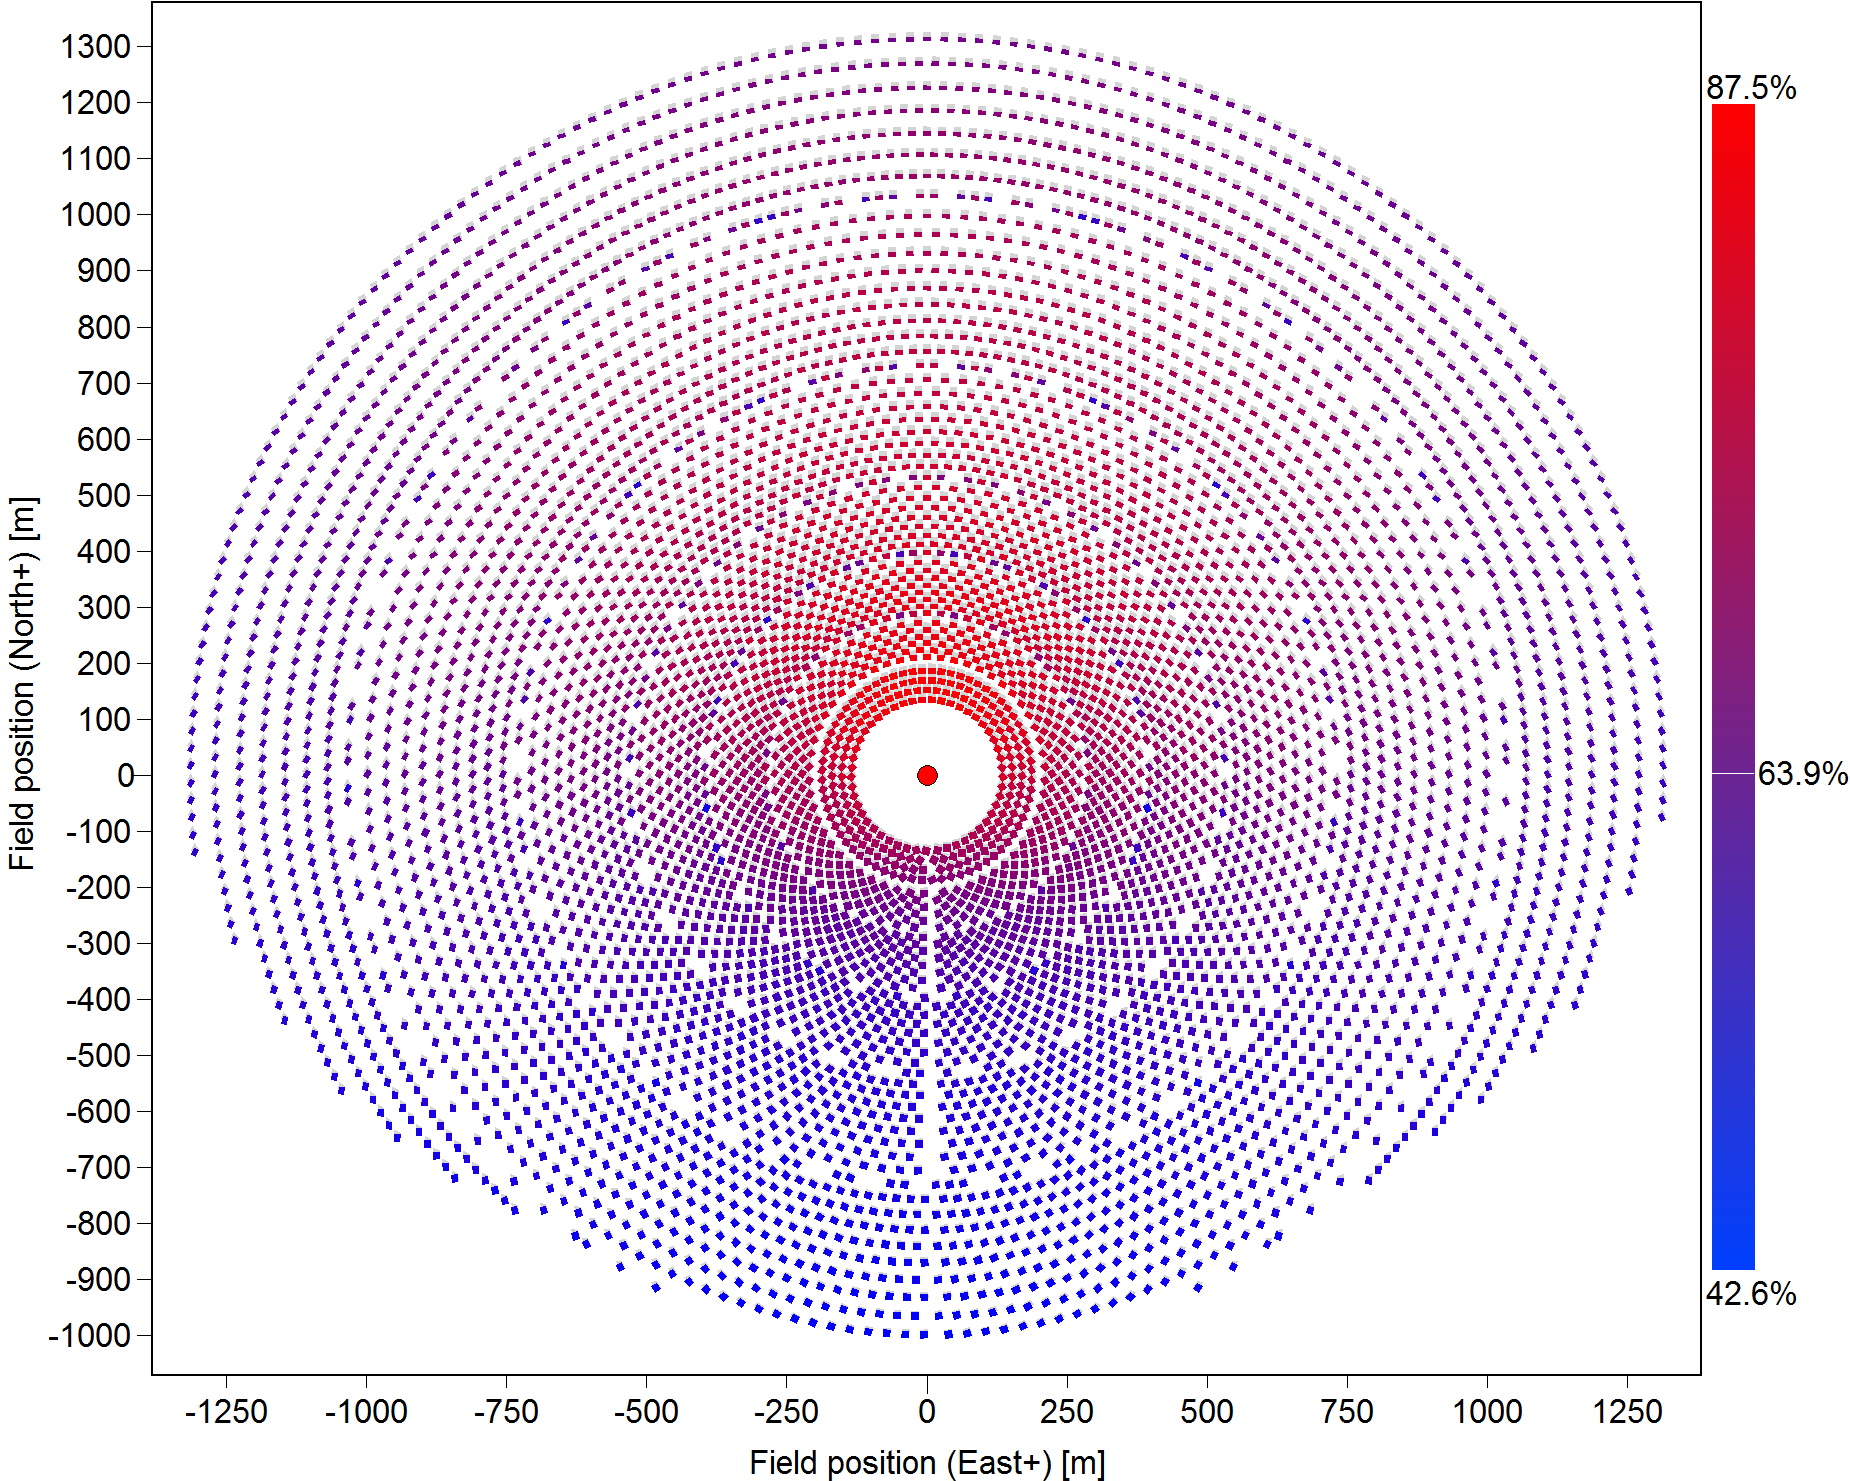
\includegraphics[width=\linewidth]{case-1}
	\caption{Case 1}
	\label{fig:cases-1}
\end{subfigure}~
\begin{subfigure}{0.48\linewidth}
	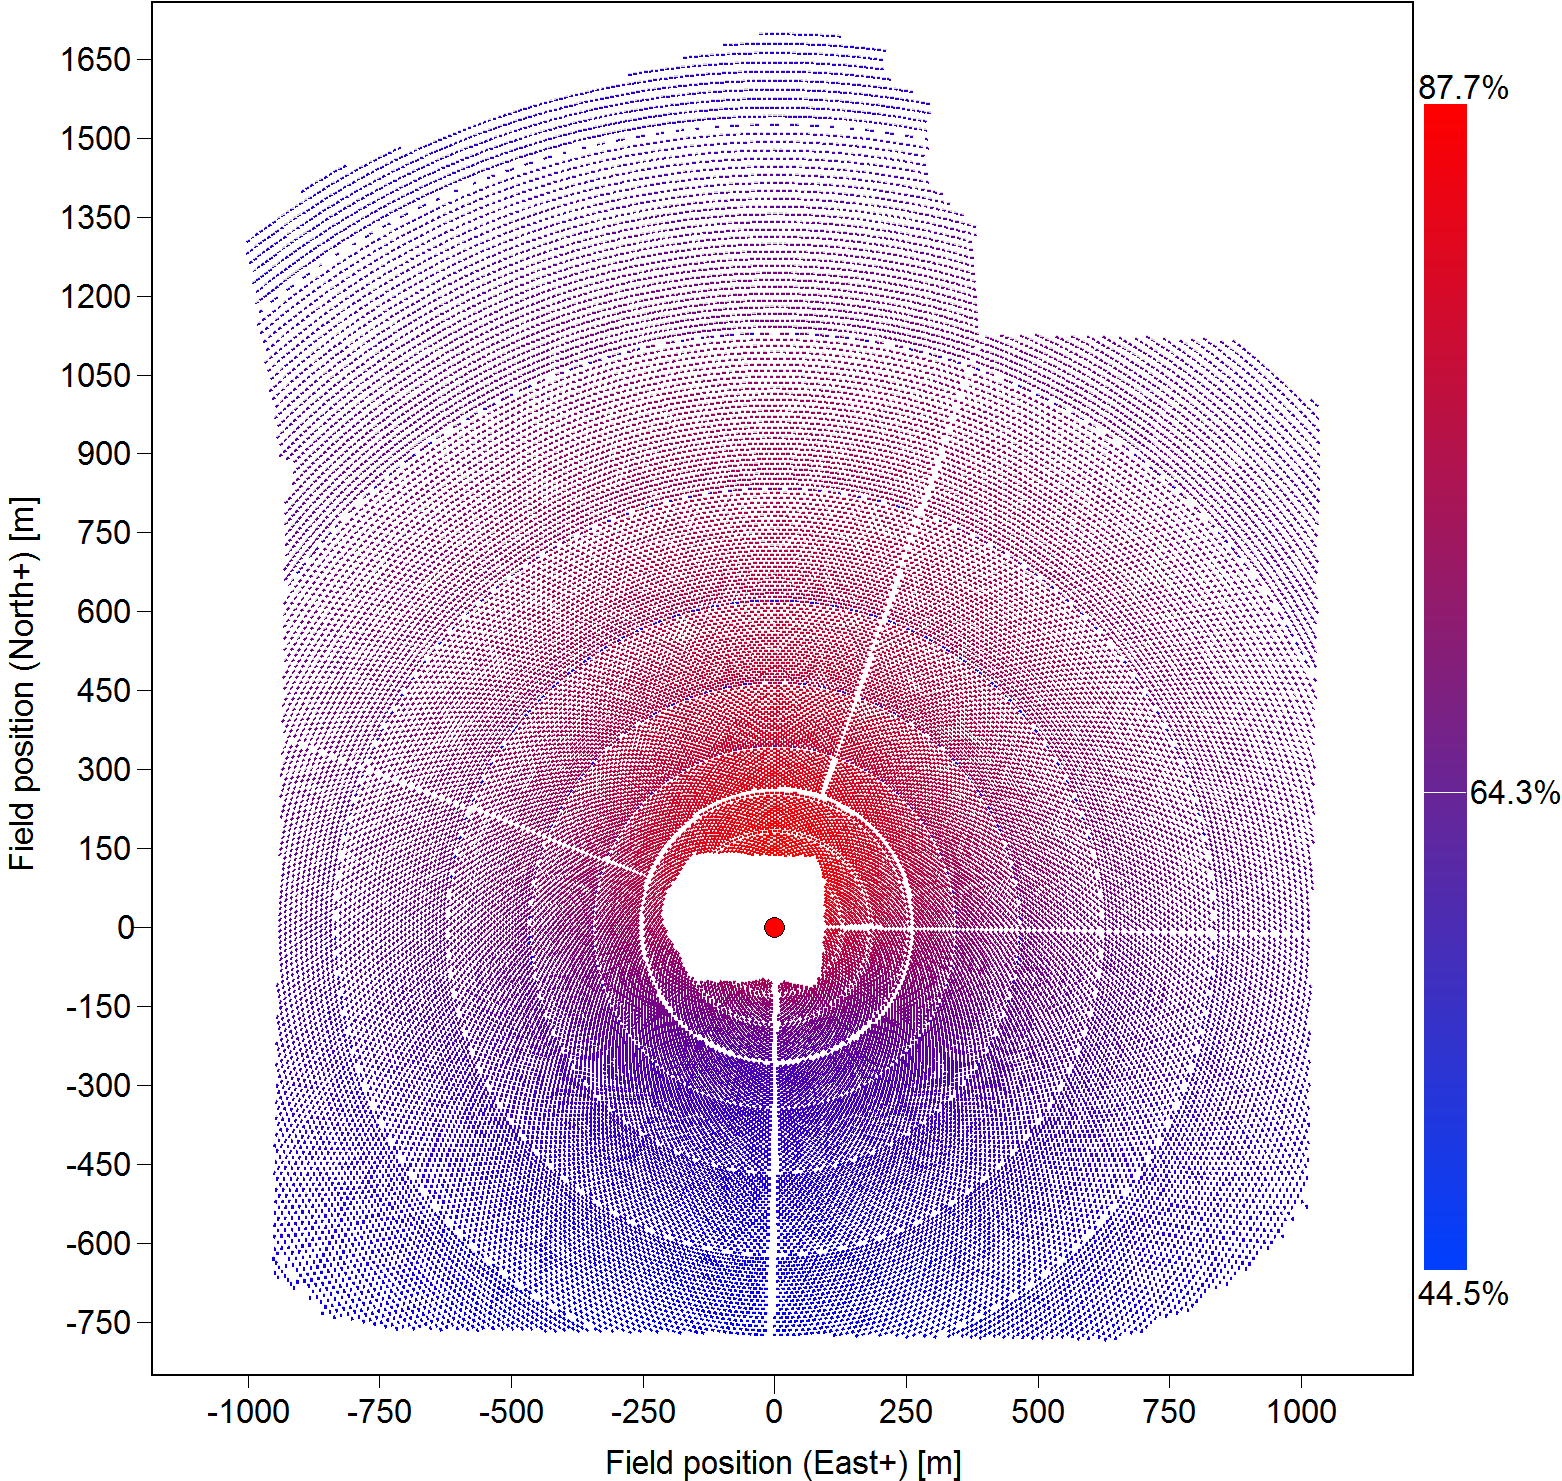
\includegraphics[width=\linewidth]{case-4}
	\caption{Case 4}
	\label{fig:cases-4}
\end{subfigure}

\begin{subfigure}{0.48\linewidth}
	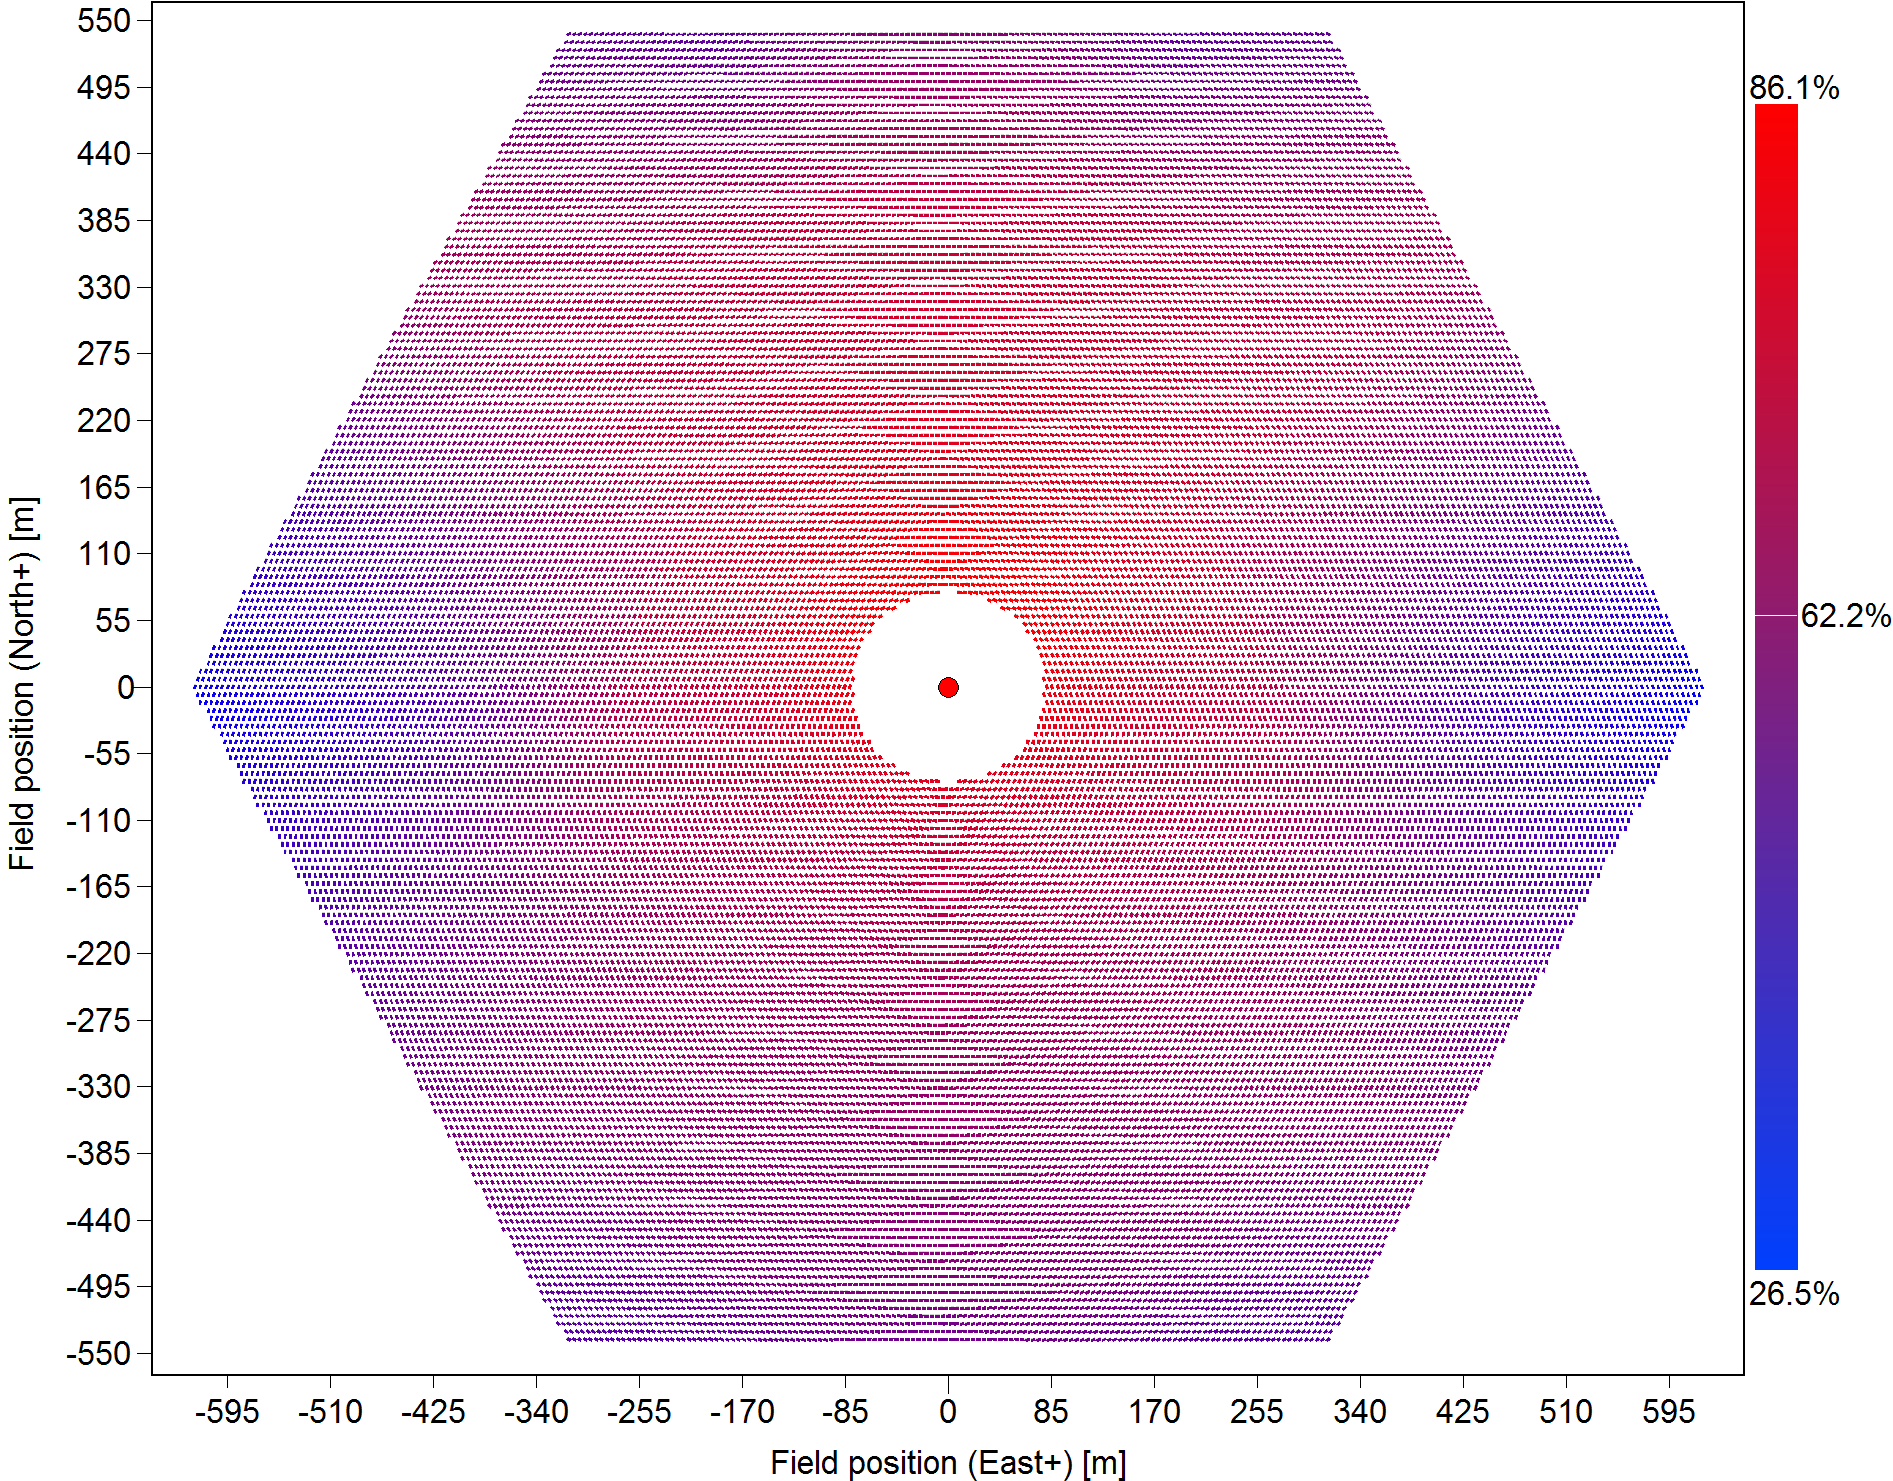
\includegraphics[width=\linewidth]{case-5}
	\caption{Case 5}
	\label{fig:cases-5}
\end{subfigure}~
\begin{subfigure}{0.48\linewidth}
	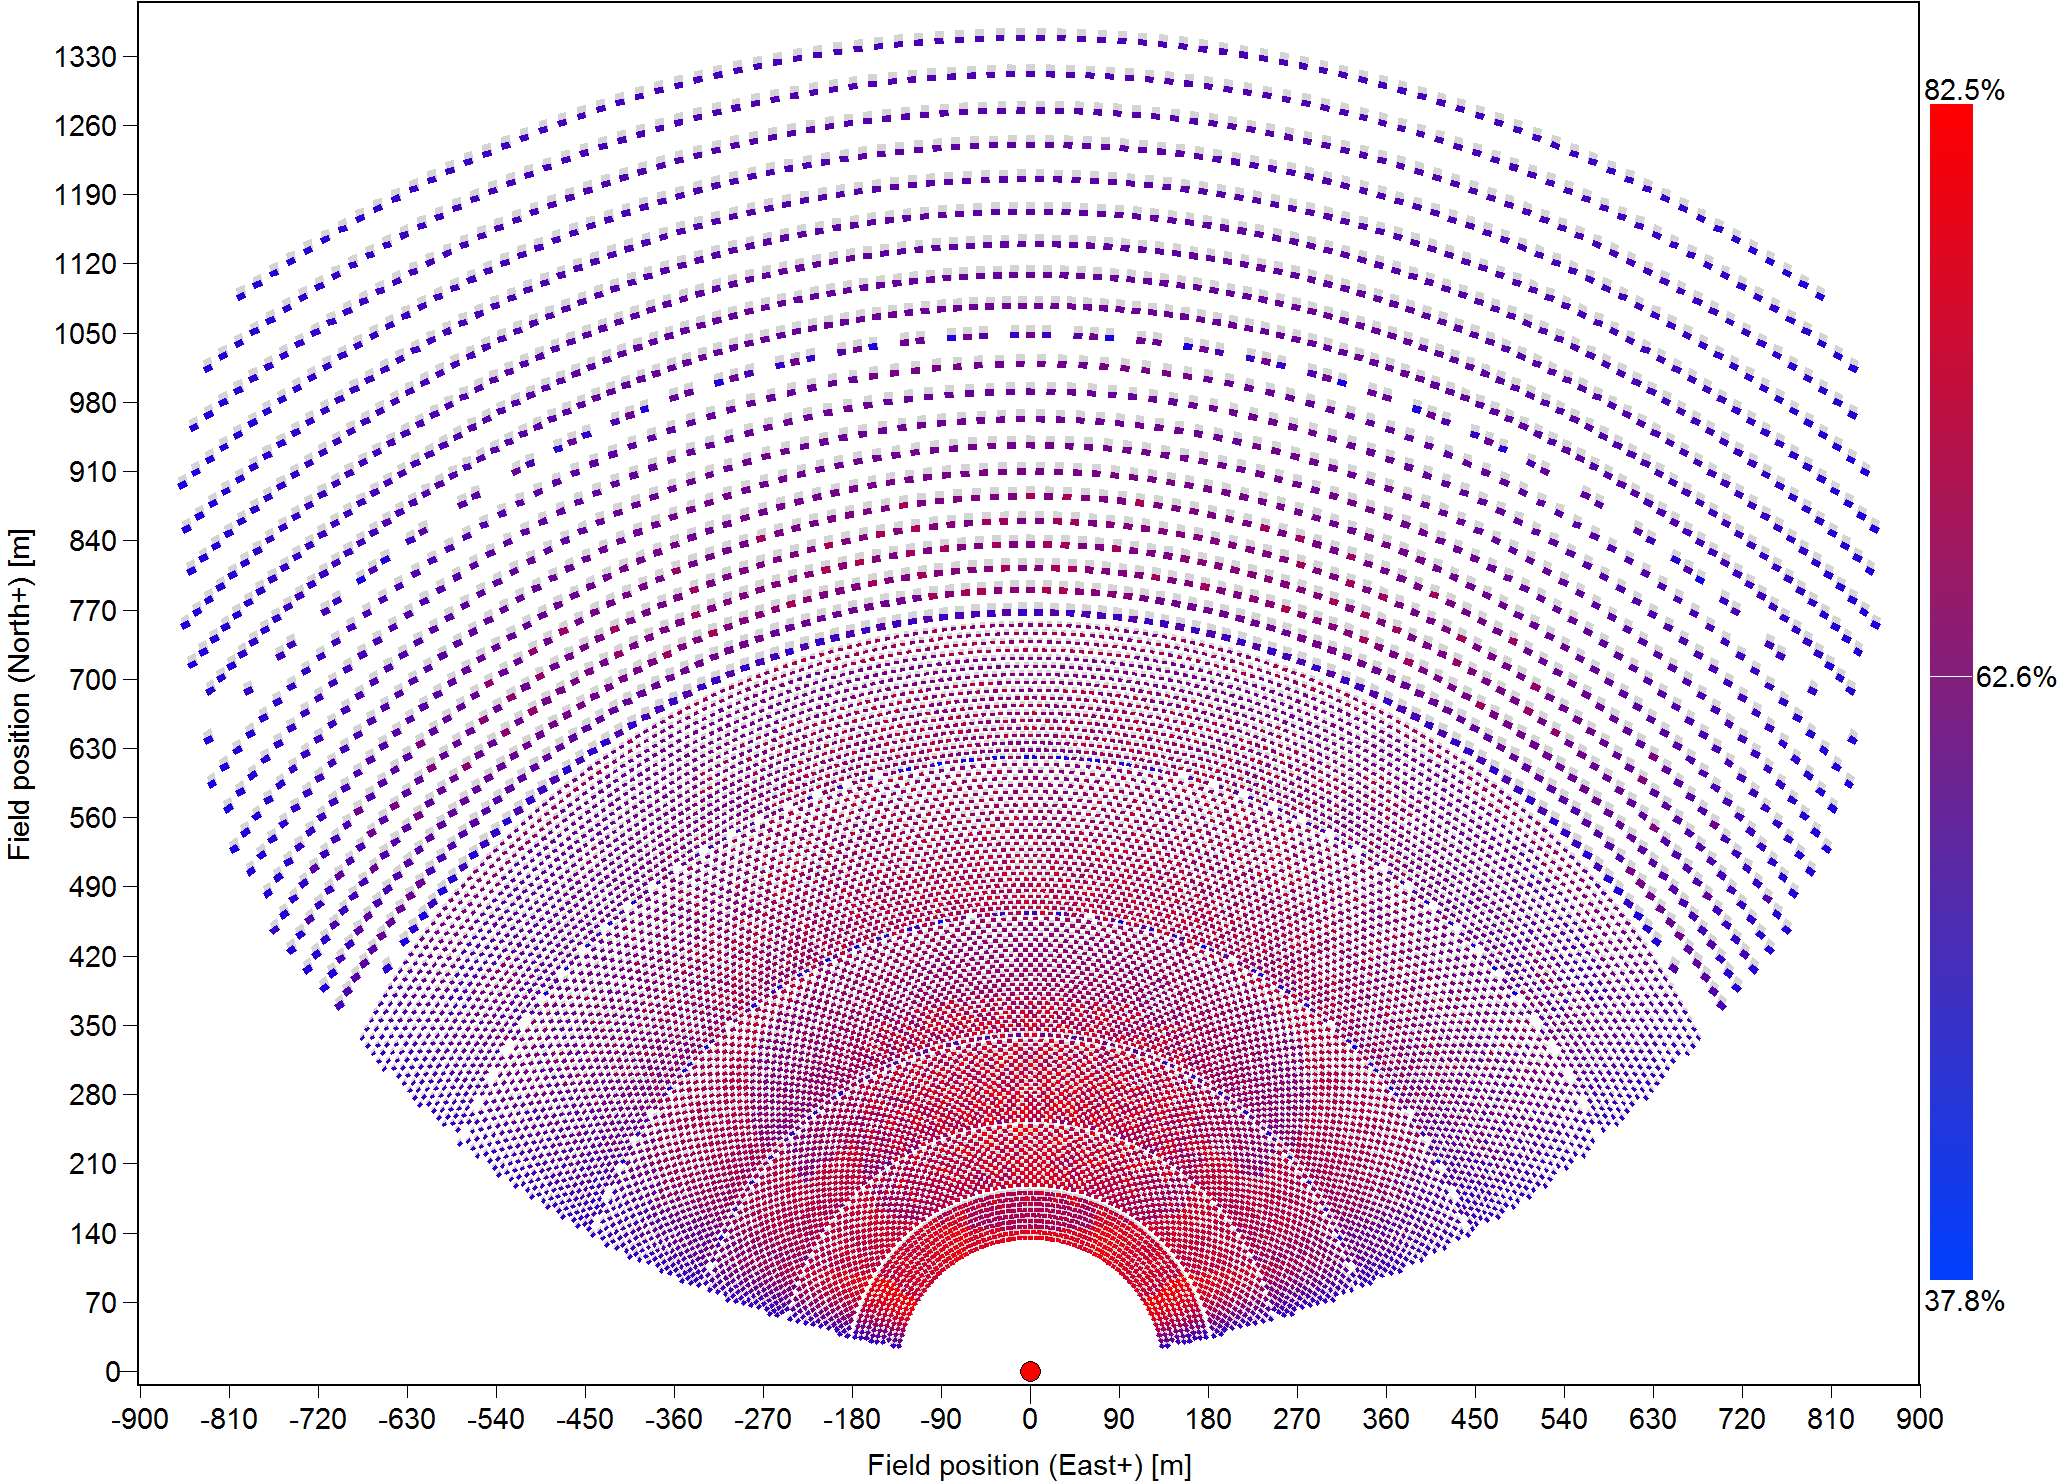
\includegraphics[width=\linewidth]{case-6}
	\caption{Case 6}
	\label{fig:cases-6}
\end{subfigure}
\caption{}
\label{fig:cases}
\end{figure}


\begin{table}
[htb]
\centering \small
\caption{Summary of test cases for SolTrace speed improvement.}
\label{tab:cases}
\begin{tabular}{c|c|L{0.4\linewidth}||c|c|>{\columncolor{yellow}}c}
\textbf{Case} & \textbf{\# Elements} & \textbf{Description} & \textbf{Base} & \textbf{Time} & \textbf{Factor} \\ %& \textbf{Factor}      \\
			  &                      &                      & \textbf{[s]}  & \textbf{[s]}  &                 \\ %& \textbf{$10^7$ rays} \\
\hline
1 & 100,512 & Default SolarPILOT case, 500MWt 
& 11,672 & 6.7 & 1,742$\times$ \\ %187486
2 & 100,512 & Same as case 1, afternoon sun position, $\theta=23^\circ,\ \alpha=253^\circ$ 
& 8,325 & 6.4 & 1,300$\times$ \\  %187547
3 & 6,282   & Default case with single-facet heliostats 
& 926.9 & 2.5 & 370$\times$ \\
4 & 95,174 & Ivanpah-like facility
& 6,531 & 9.6 & 680$\times$ \\ %187645
5 & 34,188 & Hexagonal field with regular layout
& 5,447 & 6.1 & 893$\times$ \\ %last ray 187512
6 & 79,812 & North field, mixed heliostat templates (small inner, large outer)
& 6,683 & 6.2 & 1,078$\times$ \\  %187514
\end{tabular}
\end{table}






\subsection{Verification}

Model verification is straightforward in that the improved methodology should yield exactly the same result as the original code. 
If implemented correctly, this methodology should result in any particular ray intersecting with the same optical element in the same position as the original case. 
Therefore, the methodology is verified if the calculated ray intersection table is identically reproduced after implementation. 
The ray intersections are sensitive to sequence, and a single incongruity will alter subsequent rays. 
In short, the final ray in the post-modification tool should have the same position, ray number, and attributes as the final ray in the pre-modification simulation. 
If the final rays match, all previous rays match and the methodology is verified. 
In all test cases, the ray data was replicated exactly with final rays matching. 



\subsection{Conclusions and research impact}
We have presented a methodology and implementation for improving the computational efficiency of the SolTrace ray tracing algorithm and have demonstrated the significant improvement that resulted from our effort. 
While the realized speed improvement depends on the computer architecture and the scenario under consideration, each case that we tested resulted in an improvement of at least 370$\times$, with a maximum improvement of 1,732$\times$ and an average improvement of 1,010$\times$. 
We observe that the speed improvement is most pronounced for systems with systems with higher quantities of heliostat field elements, and the improvement is independent of sun position and layout technique. 

The implications of this improvement are significant. 
Firstly, detailed ray-tracing simulations that recently required days to run, or required expensive and robust computer hardware, can now be run in a matter of seconds or minutes on readily available hardware. 
The flexibility of the ray tracing technique will allow users to quickly investigate novel heliostat or receiver geometries. 
Quick simulation turnaround allows much broader parametric and optimization studies. 

The methodology that has been developed can be implemented in ray tracing tools other than SolTrace, as it has general applicability and offers a novel approach for quickly constructing and retrieving element groups. 
In future work, we will improve the integration of the improved SolTrace engine in SolarPILOT and SAM, where the flexibility of ray-tracing can enhance the technology modeling options that are currently available. 







\end{document}